%% NEJM AI Perspective template
%% Compile: latexmk -pdf main.tex
%% Body word target: 1,200 words (NEJM AI Perspective ceiling)
%% References: <= 5; Figures: 1; Abstract: 1-2 sentences
%% Citation style: AMA numerical superscript (natbib super sort&compress)

\documentclass[11pt,a4paper]{article}
\usepackage[T1]{fontenc}\usepackage[utf8]{inputenc}\usepackage{lmodern}
\usepackage[margin=2.1cm]{geometry}
\usepackage{graphicx}\usepackage{amsmath,amssymb}\usepackage{booktabs}
\usepackage{caption}\usepackage{microtype}\usepackage{authblk}
\usepackage{xcolor}
\usepackage[colorlinks=true,citecolor=blue,linkcolor=blue,urlcolor=blue]{hyperref}
\usepackage[numbers,super,sort&compress]{natbib}
\usepackage{titlesec}
\titleformat{\section}{\fontsize{12}{14}\bfseries\sffamily}{\thesection}{0.6em}{}
\setlength{\parskip}{0.3\baselineskip}\setlength{\parindent}{0pt}

\title{\fontsize{15}{18}\bfseries\sffamily
The prompt is the protocol: a disclosure standard for clinician-investigators using agentic large language models}

\author[1,*]{Hsieh-Ting Lin, M.D.}
\affil[1]{Department of Hematology and Medical Oncology, Koo Foundation Sun Yat-Sen Cancer Center, Taipei, Taiwan. ORCID: 0009-0002-3974-4528.}
\affil[*]{Correspondence: \texttt{mail@hsiehting.com}.}
\date{}

\begin{document}
\maketitle\thispagestyle{empty}\vspace{-2em}

\noindent\textbf{Article type.} Perspective. \textbf{Body word count.} 620 (ceiling 1\,200; brevity is consistent with the journal's ``brief, accessible'' Perspective format). \textbf{References.} 5/5. \textbf{Figures.} 1/1. \textbf{Conflicts of interest.} None. \textbf{Funding.} None.

\medskip

\noindent\textbf{Abstract.} A single clinician-investigator can in 2026 assemble an end-to-end agentic-LLM research workflow on commodity tooling; current biomedical-journal AI policies classify most of what such a workflow does as prohibited, and we propose a Disclosure 2.0 standard --- prompts, model identifier, commit history, reviewer-subagent transcripts, audit log, tagged release --- under which the present Perspective and its supporting null-result case study are themselves produced.

\section{The 2026 landscape}

In 2026, two peer-reviewed \textit{Nature} papers placed autonomous agentic-LLM research at the centre of scientific publishing. Google DeepMind's Co-Scientist\citep{coscientist2026} generated, critiqued and refined biomedical hypotheses, with acute-myeloid-leukaemia drug-repurposing candidates validated \textit{in vitro}. Sakana AI's end-to-end pipeline\citep{luSakana2026} produced a manuscript that passed first-round workshop peer review under blind review; the authors' Limitations enumerate hallucinated citations and naive ideas. In parallel, a clinician with no large-lab affiliation can in 2026 assemble a workflow that performs every Co-Scientist task on commodity tooling --- one domain prompt, a handful of orchestration prompts, an open-source LLM CLI --- and produce a manuscript matched to a target journal's specifications. This Perspective and its supporting hepatocellular-carcinoma case study are the existence proof.

\section{The disclosure gap}

The biomedical-journal AI policy in current public form across the Lancet group, NEJM family and JAMA Network permits ``readability and language improvements only''\citep{lancetaipolicy2024} and prohibits using AI to generate scientific arguments, draft methodology, write literature reviews, or create new content. Read literally, the policy classifies almost every action a 2026 agentic workflow performs as prohibited. Read sympathetically, it protects against three real harms --- authorship inflation, scientific hallucination and undocumented intervention --- with rules calibrated for a 2023 generation of LLM use. The policy's intent is sound; the mechanism is mis-calibrated. Disclosure by a single-sentence acknowledgement cannot tell a reader which sentences were AI-drafted, which prompts produced them, or whether the cited literature actually exists.

\section{Disclosure 2.0}

We propose that the published unit for AI-assisted biomedical research become a tuple of six artefacts at a tagged release: (1)~the prompts that orchestrated the work, verbatim, in order, closed for edits; (2)~the model identifier with snapshot date and tool envelope; (3)~the git commit history with no force-pushes or rebases; (4)~the reviewer-subagent transcripts per round; (5)~the audit log from a sealed re-execution-plus-citation-veracity-plus-statistic-rederivation subagent; (6)~the tagged release with a persistent DOI. A minimum viable manifest (items 1, 2, 3, 6) covers the consequential audit surfaces at near-zero infrastructure cost. A vigorous human-in-the-loop school exemplified by the Academic Research Skills toolkit\citep{ars2026} argues for AI under operator supervision rather than autonomous use; the two regimes are different equilibria with different cost-of-error profiles, and Disclosure 2.0 is the disclosure layer both should share. Figure~\ref{fig:ledger} is the artefact ledger of the present Perspective.

\begin{figure}[h]\centering
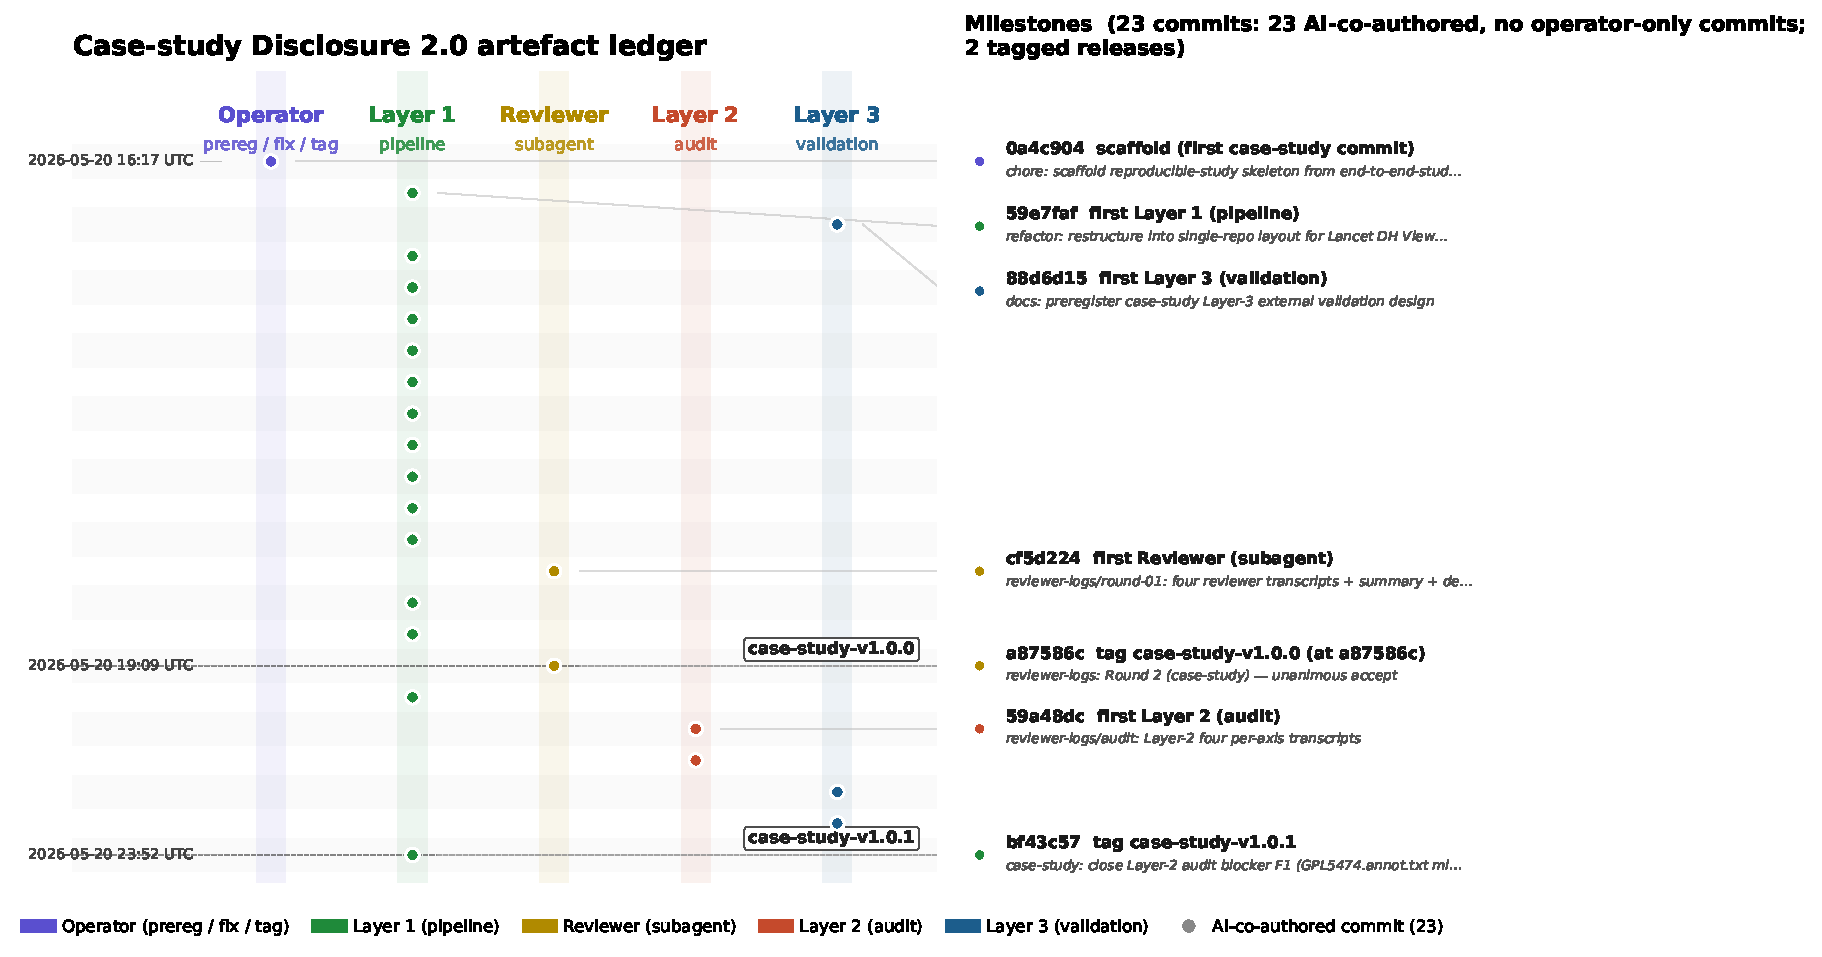
\includegraphics[width=0.85\textwidth]{figures/fig1-artifact-ledger.pdf}
\caption{Disclosure 2.0 artefact ledger for the supporting case study, regenerated from \texttt{git log} on each release tag. Markers: commits coloured by AI-co-authorship status, reviewer-subagent rounds, audit checkpoints, and tagged release.}\label{fig:ledger}\end{figure}

\section{The supporting null}

The supporting case study runs Disclosure 2.0 on a hepatocellular-carcinoma overall-survival stratification problem outside the operator's clinical sub-specialty. Layer 1, a single autonomous Claude Code session, produced a 50-gene risk score with development-cohort paired-optimism $\Delta C$-index = 0.063 (95\,\% CI [0.003, 0.113], $n=366$). Layer 2 (a sealed audit subagent) filed twelve substantive findings including one blocker (a required annotation file not downloaded by the data-prep script) and two high-severity (an abstract estimator that disagrees with the Methods specification; a stratified-vs-stage-adjusted HR discrepancy). Layer 3 (the operator's preregistered\citep{repoprereg} external validation against held-out GSE14520 and GSE76427, pooled $n=333$, 107 events) returned $\Delta C = 0.006$, 95\,\% CI [$-0.008$, $0.030$] --- primary hypothesis \emph{not rejected}; calibration drifts from 1.1 at 1\,y to 1.9 at 5\,y; IDI~$\approx 0$. The development-cohort positive does not transport. The null is the headline; the manifest preserves it together with the twelve audit findings as evidence the regime makes its own failure modes visible.

\section{Recommendation}

NEJM AI and the wider biomedical-journal community should pilot Disclosure 2.0 as an alternative submission track for AI-deep manuscripts, with a JSON-schema manifest (committed at the repository root and validated at submission via PDF attachment plus linked DOI) and a 90-day trial in which five to ten submissions per quarter attach the manifest. The Perspective the reviewer is reading was assembled under exactly that standard; every artefact the manifest would require is publicly archived at \texttt{https://github.com/htlin222/end-to-end} under MIT licence at tag \texttt{viewpoint-nejmai-v1.0.0}, with a Zenodo DOI minted on tag push. The medium is the message; whatever the editorial decision, the artefact stands.

%% -------------------------------------------------------------------------
\section*{Declarations}
\noindent\textbf{Conflicts of interest.} The author declares no competing interests. \textbf{Funding.} None. \textbf{Role of the funding source.} No funder; full repository access and final submission decision rest with the author. \textbf{AI usage.} Manuscript drafted with Anthropic Claude (Opus 4.7, 1M-context variant) via the Claude Code CLI; per-step disclosure log at \texttt{docs/ai-usage-disclosure.md} in the linked repository. No AI tool is listed as an author; no AI tool generated figures. \textbf{Data and code availability.} All artefacts at \texttt{https://github.com/htlin222/end-to-end} (MIT licence; tag \texttt{viewpoint-nejmai-v1.0.0}).

\bibliographystyle{vancouver}
\bibliography{references}
\end{document}
